%%%%%%%%%%%%%%%%%%%%%%%%%%%%%%%%%%%%%%%%%
% Short Sectioned Assignment
% LaTeX Template
% Version 1.0 (5/5/12)
%
% This template has been downloaded from:
% http://www.LaTeXTemplates.com
%
% Original author:
% Frits Wenneker (http://www.howtotex.com)
%
% License:
% CC BY-NC-SA 3.0 (http://creativecommons.org/licenses/by-nc-sa/3.0/)
%
%%%%%%%%%%%%%%%%%%%%%%%%%%%%%%%%%%%%%%%%%

%----------------------------------------------------------------------------------------
%	PACKAGES AND OTHER DOCUMENT CONFIGURATIONS
%----------------------------------------------------------------------------------------

\documentclass[paper=a4, fontsize=11pt]{scrartcl} % A4 paper and 11pt font size

\usepackage[T1]{fontenc} % Use 8-bit encoding that has 256 glyphs
\usepackage{fourier} % Use the Adobe Utopia font for the document - comment this line to return to the LaTeX default
\usepackage[english]{babel} % English language/hyphenation
\usepackage{amsmath,amsfonts,amsthm} % Math packages

\usepackage{lipsum} % Used for inserting dummy 'Lorem ipsum' text into the template

\usepackage{sectsty} % Allows customizing section commands
\allsectionsfont{\centering \normalfont\scshape} % Make all sections centered, the default font and small caps

\usepackage{graphicx}
\usepackage{float}

\usepackage{fancyhdr} % Custom headers and footers
\pagestyle{fancyplain} % Makes all pages in the document conform to the custom headers and footers
\fancyhead{} % No page header - if you want one, create it in the same way as the footers below
\fancyfoot[L]{} % Empty left footer
\fancyfoot[C]{} % Empty center footer
\fancyfoot[R]{\thepage} % Page numbering for right footer
\renewcommand{\headrulewidth}{0pt} % Remove header underlines
\renewcommand{\footrulewidth}{0pt} % Remove footer underlines
\setlength{\headheight}{13.6pt} % Customize the height of the header

\numberwithin{equation}{section} % Number equations within sections (i.e. 1.1, 1.2, 2.1, 2.2 instead of 1, 2, 3, 4)
\numberwithin{figure}{section} % Number figures within sections (i.e. 1.1, 1.2, 2.1, 2.2 instead of 1, 2, 3, 4)
\numberwithin{table}{section} % Number tables within sections (i.e. 1.1, 1.2, 2.1, 2.2 instead of 1, 2, 3, 4)

\setlength\parindent{0pt} % Removes all indentation from paragraphs - comment this line for an assignment with lots of text


%----------------------------------------------------------------------------------------
%	TITLE SECTION
%----------------------------------------------------------------------------------------

\newcommand{\horrule}[1]{\rule{\linewidth}{#1}} % Create horizontal rule command with 1 argument of height

\title{	
\normalfont \normalsize 
\textsc{McGill University} \\ [25pt] % Your university, school and/or department name(s)
\horrule{0.5pt} \\[0.4cm] % Thin top horizontal rule
\huge Homework 1 \\ % The assignment title
\horrule{2pt} \\[0.5cm] % Thick bottom horizontal rule
}

\author{
    Nabil Chowdhury \\
    \small{ID: 260622155} \\
    \small{COMP 424} \\
} % Your name

\begin{document}
\maketitle % Print the title
%--------------
%	PROBLEM 1
%--------------
\section{Question 1: Six Puzzle}
\subsection{PART A: Solution paths for various search algorithms}
The paths were all found programmatically using Java. Please see Question1.java for implementation details. \\
Note: As specified by the assignment, neighboring states are explored by lowest-valued piece moved. For example, if the valid moves are moving 2 and 4, then moving the 2 is explored first.
\subsubsection{Breadth-First Search}
\begin{center}
[[1, 4, 2][5, 3, 0]] ---> [[1, 4, 2][5, 0, 3]] ---> [[1, 0, 2][5, 4, 3]] ---> [[0, 1, 2][5, 4, 3]]
\end{center}

\subsubsection{Uniform Cost Search}
\begin{center}
[[1, 4, 2][5, 3, 0]] ---> [[1, 4, 2][5, 0, 3]] ---> [[1, 0, 2][5, 4, 3]] ---> [[0, 1, 2][5, 4, 3]]
\end{center}

\subsubsection{Depth-First Search}
\begin{center}
[[1, 4, 2][5, 3, 0]] ---> [[1, 4, 0][5, 3, 2]] ---> [[1, 0, 4][5, 3, 2]] ---> [[0, 1, 4][5, 3, 2]] ---> [[5, 1, 4][0, 3, 2]] ---> [[5, 1, 4][3, 0, 2]] ---> [[5, 0, 4][3, 1, 2]] ---> [[5, 4, 0][3, 1, 2]] ---> [[5, 4, 2][3, 1, 0]] ---> [[5, 4, 2][3, 0, 1]] ---> [[5, 4, 2][0, 3, 1]] ---> [[0, 4, 2][5, 3, 1]] ---> [[4, 0, 2][5, 3, 1]] ---> [[4, 2, 0][5, 3, 1]] ---> [[4, 2, 1][5, 3, 0]] ---> [[4, 2, 1][5, 0, 3]] ---> [[4, 0, 1][5, 2, 3]] ---> [[4, 1, 0][5, 2, 3]] ---> [[4, 1, 3][5, 2, 0]] ---> [[4, 1, 3][5, 0, 2]] ---> [[4, 0, 3][5, 1, 2]] ---> [[4, 3, 0][5, 1, 2]] ---> [[4, 3, 2][5, 1, 0]] ---> [[4, 3, 2][5, 0, 1]] ---> [[4, 3, 2][0, 5, 1]] ---> [[0, 3, 2][4, 5, 1]] ---> [[3, 0, 2][4, 5, 1]] ---> [[3, 2, 0][4, 5, 1]] ---> [[3, 2, 1][4, 5, 0]] ---> [[3, 2, 1][4, 0, 5]] ---> [[3, 0, 1][4, 2, 5]] ---> [[3, 1, 0][4, 2, 5]] ---> [[3, 1, 5][4, 2, 0]] ---> [[3, 1, 5][4, 0, 2]] ---> [[3, 0, 5][4, 1, 2]] ---> [[0, 3, 5][4, 1, 2]] ---> [[4, 3, 5][0, 1, 2]] ---> [[4, 3, 5][1, 0, 2]] ---> [[4, 3, 5][1, 2, 0]] ---> [[4, 3, 0][1, 2, 5]] ---> [[4, 0, 3][1, 2, 5]] ---> [[4, 2, 3][1, 0, 5]] ---> [[4, 2, 3][0, 1, 5]] ---> [[0, 2, 3][4, 1, 5]] ---> [[2, 0, 3][4, 1, 5]] ---> [[2, 1, 3][4, 0, 5]] ---> [[2, 1, 3][0, 4, 5]] ---> [[0, 1, 3][2, 4, 5]] ---> [[1, 0, 3][2, 4, 5]] ---> [[1, 3, 0][2, 4, 5]] ---> [[1, 3, 5][2, 4, 0]] ---> [[1, 3, 5][2, 0, 4]] ---> [[1, 3, 5][0, 2, 4]] ---> [[0, 3, 5][1, 2, 4]] ---> [[3, 0, 5][1, 2, 4]] ---> [[3, 2, 5][1, 0, 4]] ---> [[3, 2, 5][0, 1, 4]] ---> [[0, 2, 5][3, 1, 4]] ---> [[2, 0, 5][3, 1, 4]] ---> [[2, 1, 5][3, 0, 4]] ---> [[2, 1, 5][0, 3, 4]] ---> [[0, 1, 5][2, 3, 4]] ---> [[1, 0, 5][2, 3, 4]] ---> [[1, 5, 0][2, 3, 4]] ---> [[1, 5, 4][2, 3, 0]] ---> [[1, 5, 4][2, 0, 3]] ---> [[1, 5, 4][0, 2, 3]] ---> [[0, 5, 4][1, 2, 3]] ---> [[5, 0, 4][1, 2, 3]] ---> [[5, 2, 4][1, 0, 3]] ---> [[5, 2, 4][0, 1, 3]] ---> [[0, 2, 4][5, 1, 3]] ---> [[2, 0, 4][5, 1, 3]] ---> [[2, 1, 4][5, 0, 3]] ---> [[2, 1, 4][5, 3, 0]] ---> [[2, 1, 0][5, 3, 4]] ---> [[2, 0, 1][5, 3, 4]] ---> [[0, 2, 1][5, 3, 4]] ---> [[5, 2, 1][0, 3, 4]] ---> [[5, 2, 1][3, 0, 4]] ---> [[5, 0, 1][3, 2, 4]] ---> [[0, 5, 1][3, 2, 4]] ---> [[3, 5, 1][0, 2, 4]] ---> [[3, 5, 1][2, 0, 4]] ---> [[3, 5, 1][2, 4, 0]] ---> [[3, 5, 0][2, 4, 1]] ---> [[3, 0, 5][2, 4, 1]] ---> [[0, 3, 5][2, 4, 1]] ---> [[2, 3, 5][0, 4, 1]] ---> [[2, 3, 5][4, 0, 1]] ---> [[2, 0, 5][4, 3, 1]] ---> [[0, 2, 5][4, 3, 1]] ---> [[4, 2, 5][0, 3, 1]] ---> [[4, 2, 5][3, 0, 1]] ---> [[4, 2, 5][3, 1, 0]] ---> [[4, 2, 0][3, 1, 5]] ---> [[4, 0, 2][3, 1, 5]] ---> [[4, 1, 2][3, 0, 5]] ---> [[4, 1, 2][0, 3, 5]] ---> [[0, 1, 2][4, 3, 5]] ---> [[1, 0, 2][4, 3, 5]] ---> [[1, 2, 0][4, 3, 5]] ---> [[1, 2, 5][4, 3, 0]] ---> [[1, 2, 5][4, 0, 3]] ---> [[1, 0, 5][4, 2, 3]] ---> [[0, 1, 5][4, 2, 3]] ---> [[4, 1, 5][0, 2, 3]] ---> [[4, 1, 5][2, 0, 3]] ---> [[4, 0, 5][2, 1, 3]] ---> [[0, 4, 5][2, 1, 3]] ---> [[2, 4, 5][0, 1, 3]] ---> [[2, 4, 5][1, 0, 3]] ---> [[2, 4, 5][1, 3, 0]] ---> [[2, 4, 0][1, 3, 5]] ---> [[2, 0, 4][1, 3, 5]] ---> [[0, 2, 4][1, 3, 5]] ---> [[1, 2, 4][0, 3, 5]] ---> [[1, 2, 4][3, 0, 5]] ---> [[1, 0, 4][3, 2, 5]] ---> [[0, 1, 4][3, 2, 5]] ---> [[3, 1, 4][0, 2, 5]] ---> [[3, 1, 4][2, 0, 5]] ---> [[3, 0, 4][2, 1, 5]] ---> [[0, 3, 4][2, 1, 5]] ---> [[2, 3, 4][0, 1, 5]] ---> [[2, 3, 4][1, 0, 5]] ---> [[2, 3, 4][1, 5, 0]] ---> [[2, 3, 0][1, 5, 4]] ---> [[2, 0, 3][1, 5, 4]] ---> [[0, 2, 3][1, 5, 4]] ---> [[1, 2, 3][0, 5, 4]] ---> [[1, 2, 3][5, 0, 4]] ---> [[1, 0, 3][5, 2, 4]] ---> [[0, 1, 3][5, 2, 4]] ---> [[5, 1, 3][0, 2, 4]] ---> [[5, 1, 3][2, 0, 4]] ---> [[5, 0, 3][2, 1, 4]] ---> [[5, 3, 0][2, 1, 4]] ---> [[5, 3, 4][2, 1, 0]] ---> [[5, 3, 4][2, 0, 1]] ---> [[5, 3, 4][0, 2, 1]] ---> [[0, 3, 4][5, 2, 1]] ---> [[3, 0, 4][5, 2, 1]] ---> [[3, 2, 4][5, 0, 1]] ---> [[3, 2, 4][5, 1, 0]] ---> [[3, 2, 0][5, 1, 4]] ---> [[3, 0, 2][5, 1, 4]] ---> [[3, 1, 2][5, 0, 4]] ---> [[3, 1, 2][5, 4, 0]] ---> [[3, 1, 0][5, 4, 2]] ---> [[3, 0, 1][5, 4, 2]] ---> [[0, 3, 1][5, 4, 2]] ---> [[5, 3, 1][0, 4, 2]] ---> [[5, 3, 1][4, 0, 2]] ---> [[5, 3, 1][4, 2, 0]] ---> [[5, 3, 0][4, 2, 1]] ---> [[5, 0, 3][4, 2, 1]] ---> [[5, 2, 3][4, 0, 1]] ---> [[5, 2, 3][4, 1, 0]] ---> [[5, 2, 0][4, 1, 3]] ---> [[5, 0, 2][4, 1, 3]] ---> [[5, 1, 2][4, 0, 3]] ---> [[5, 1, 2][0, 4, 3]] ---> [[0, 1, 2][5, 4, 3]]
\end{center}

\subsubsection{Iterative Deepening Search}
Iterative Deepening Search does not find solutions for depths 0 to 3. This makes sense since the shortest solution path is at depth 4.
\begin{center}
[[1, 4, 2][5, 3, 0]] ---> [[1, 4, 2][5, 0, 3]] ---> [[1, 0, 2][5, 4, 3]] ---> [[0, 1, 2][5, 4, 3]]
\end{center}

\subsection{Part B: Is Manhattan distance still admissible for the new cost scheme?}
From class, we know that the Manhattan distance is admissible under the unit cost scheme where moving to a neighboring state costs 1. Under this new cost scheme, moving to a neighboring state costs the value of the piece moved. The lowest piece on the board is 1, and so the Manhattan distance heuristic is still admissible since the new cost scheme \(\geq\) the unit cost scheme, since it is lower bounded by the unit cost scheme. Mathematically, we have the following: \\
\newline
\textit{h(n) = Manhattan distance heuristic \\}
\textit{u(n) = unit cost scheme \\}
\textit{u'(n) = new cost scheme \\}
\textit{S = The state space}
\[h(n) <= u(n) <= u'(n)\ \forall n \in S \]

\subsection{Part C: Design an admissible heuristic that dominates the heuristic from Part B under the same cost scheme}
We say that a heuristic \textit{h\textsubscript{2}(n)} dominates \textit{h\textsubscript{1}(n)} if \textit{h\textsubscript{2}(n)} \(\geq\) \textit{h\textsubscript{1}(n)} \(\forall n\) and both heuristics are admissible. The Manhattan distance of a piece from its current state to goal state can be multiplied by the value of the piece to get a heuristic that dominates the original heuristic.\\
\newline
Original Manhattan distance heuristic: \\
\textit{Let P be the highest valued piece on the board (i.e. the board has piece from 1 to P). \\}
\textit{Let g\textsubscript{xi} be the x coordinate of piece i in the goal board state. \\}
\textit{Let g\textsubscript{yi} be the y coordinate of piece i in the goal board state. \\}
\textit{Let c\textsubscript{xi} be the x coordinate of piece i in the current board state. \\}
\textit{Let c\textsubscript{yi} be the y coordinate of piece i in the current board state. \\}
$$\sum_{i=1}^{P} |g_{xi} - c_{xi}| + |g_{yi} - c_{yi}| = h$$

New dominant heuristic:
$$\sum_{i=1}^{P} i\times(|g_{xi} - c_{xi}| + |g_{yi} - c_{yi}|) = h'$$

This new heuristic dominates the old heuristic for 2 reasons: \\
i) \textit{h'} \(\geq\) \textit{h} since we are multiplying by \textit{i} \(\geq\) \textit{1} \\
ii) \textit{h'} is still admissible under the new cost scheme since we know in the unit cost case, the Manhattan distance is a lower bound on the actual cost. Similarly, the new cost scheme poses a greater cost than \textit{h'} since we cannot actually move a piece directly to its goal state since there may be other pieces in the way. Thus, more moves are required than what Manhattan distance assumes.

\subsection{Part D: New cost scheme in which moving pieces to the left or right costs 2, whereas
moving pieces up or down costs 0.5}
Under this new cost scheme, it is easy to find an example showing that the Manhattan distance is not admissible: \\
\begin{center}
[[5, 1, 2][0, 4, 3]] -- 0.5 --> [[0, 1, 2][5, 4, 3]]
\end{center}

In the above example, the goal state can be reached by moving the 5 down into the empty cell. The actual cost is 0.5 whereas the Manhattan distance cost is just 1. Therefore, there exists a state where \(h(n) \geq cost(n)\), and so \textit{h(n)} is not admissible.

\section{Question 2: Search Algorithms}
\subsection{Part A: Describe a state space in which iterative deepening search performs much worse than depth-first search}

Consider a state space where the goal state is found by DFS without the need for branching. In other words, the goal state is at a large depth \textit{d}, but DFS can find it in linear time (see diagram below). In such a case, iterative deepening will perform much worse than DFS since it will not get to depth \textit{d} until it fully exhausts the previous \textit{d - 1} levels, whereas DFS, with the right choice of neighbors, can get there in linear time. Here is an example of such a search tree: 
\begin{figure}[H]
    \includegraphics[width=\linewidth]{searchtree.png}
\end{figure}

\subsection{Part B: T/F: Breadth-first search is a special case of uniform-cost search/}
True. BFS is Uniform-cost search with unit cost (transition cost is 1). This can be seen by noticing that BFS explores the search tree layer by layer (it explores all nodes at depth \textit{d} before exploring depth \textit{d + 1}). Uniform cost search uses a priority queue where the cost so far is the priority. With a transition cost of 1, all neighbors are pushed to the back of the priority queue since the cost of all neighbors is the cost of the current node plus 1, and this emulates standard BFS.

\subsection{Part C: T/F: Depth-first search is a special case of best-first tree search}
True. Best-first tree search becomes the standard Depth-first search if the heuristic \textit{h(n) = -depth(n)}. The child \textit{n'} of a node \textit{n} with depth \textit{depth(n)}, has depth \textit{depth(n)} + 1. Evaluating \textit{h(n')} gives us \textit{-(depth(n) + 1)}. Since \textit{h(n') < h(n)}, \textit{n'} is now at the front of the priority queue, and will be explored next.

\subsection{Part D: T/F: Uniform cost search is a special case of A* search}
True. A* search is a greedy search with respect to the function \textit{f(n) = g(n) + h(n)}, where \textit{g} is the cost of the path so far, and \textit{h} is the admissible heuristic. Since A* expands nodes with the lowest \textit{f} first, we can set \textit{h(n) = 0} \(\forall\) \textit{n}. Now, \textit{f} is simply the cost of the path so far, and this is exactly uniform cost search.

\section{Question 3: Optimization}
\subsection{Part A: Hill climbing}

\begin{center}
\begin{tabular}{ |c|c|c|c|c| } 
	\hline
	\textbf{Step size} & \textbf{X\textsubscript{0}} & \textbf{Iterations} & \textbf{X*} & \textbf{Y*} \\ 
	\hline
    0.01 & 0 & 175 & 1.7400000000000013 & 0.3960158890993247 \\
    0.01 & 1 & 75 & 1.7400000000000007 & 0.39601588909932467 \\
    0.01 & 2 & 27 & 1.7399999999999998 & 0.3960158890993246 \\
    0.01 & 3 & 127 & 1.740000000000021 & 0.3960158890993246 \\
    0.01 & 4 & 5 & 3.960000000000001 & 0.3341097537786864 \\
    0.01 & 5 & 33 & 5.319999999999993 & 0.31049661129613665 \\
    0.01 & 6 & 40 & 6.389999999999992 & 0.2961072260386306 \\
    0.01 & 7 & 32 & 7.309999999999993 & 0.28572281037034464 \\
    0.01 & 8 & 13 & 8.119999999999997 & 0.2777774823660866 \\
    0.01 & 9 & 15 & 8.860000000000003 & 0.27132890618876104 \\
    0.01 & 10 & 1 & 10 & -0.06891263333078856 \\
    0.02 & 0 & 88 & 1.740000000000001 & 0.39601588909932467 \\
    0.02 & 1 & 38 & 1.7400000000000007 & 0.39601588909932467 \\
    0.02 & 2 & 14 & 1.7399999999999998 & 0.3960158890993246 \\
    0.02 & 3 & 64 & 1.7399999999999989 & 0.3960158890993247 \\
    0.02 & 4 & 3 & 3.96 & 0.3341097537786864 \\
    0.02 & 5 & 17 & 5.319999999999993 & 0.31049661129613665 \\
    0.02 & 6 & 20 & 6.379999999999992 & 0.29554413206295477 \\
    0.02 & 7 & 16 & 7.299999999999994 & 0.28536751773684105 \\
    0.02 & 8 & 7 & 8.119999999999997 & 0.2777774823660866 \\
    0.02 & 9 & 8 & 8.860000000000003 & 0.27132890618876104 \\
    0.02 & 10 & 1 & 10 & -0.06891263333078856 \\
    0.03 & 0 & 59 & 1.7400000000000013 & 0.3960158890993247 \\
    0.03 & 1 & 26 & 1.7500000000000007 & 0.39595546426910133 \\
    0.03 & 2 & 10 & 1.7299999999999998 & 0.3959593690679719 \\
    0.03 & 3 & 43 & 1.7400000000000062 & 0.3960158890993246 \\
    0.03 & 4 & 2 & 3.97 & 0.33381970937891065 \\
    0.03 & 5 & 12 & 5.330000000000003 & 0.30967579571438547 \\
    0.03 & 6 & 14 & 6.390000000000003 & 0.29610722603863054 \\
    0.03 & 7 & 11 & 7.3000000000000025 & 0.285367517736842 \\
    0.03 & 8 & 5 & 8.119999999999997 & 0.2777774823660866 \\
    0.03 & 9 & 6 & 8.850000000000003 & 0.26986547867397453 \\
    0.03 & 10 & 1 & 10 & -0.06891263333078856 \\
    0.04 & 0 & 44 & 1.7200000000000009 & 0.395787755789096 \\
    0.04 & 1 & 19 & 1.7200000000000006 & 0.395787755789096 \\
    0.04 & 2 & 8 & 1.7199999999999998 & 0.39578775578909586 \\
    0.04 & 3 & 33 & 1.7199999999999989 & 0.3957877557890959 \\
    0.04 & 4 & 2 & 3.96 & 0.3341097537786864 \\
    0.04 & 5 & 9 & 5.32 & 0.3104966112961364 \\
    0.04 & 6 & 11 & 6.4 & 0.2954619405059111 \\
    0.04 & 7 & 9 & 7.32 & 0.28455196632004937 \\
    0.04 & 8 & 4 & 8.119999999999997 & 0.2777774823660866 \\
    0.04 & 9 & 4 & 8.880000000000003 & 0.267870590383232 \\
    0.04 & 10 & 1 & 10 & -0.06891263333078856 \\
    0.05 & 0 & 36 & 1.7500000000000009 & 0.39595546426910133 \\
    0.05 & 1 & 16 & 1.7500000000000007 & 0.39595546426910133 \\
    0.05 & 2 & 6 & 1.7499999999999998 & 0.3959554642691013 \\
    0.05 & 3 & 26 & 1.7500000000000033 & 0.3959554642691012 \\
    0.05 & 4 & 2 & 3.95 & 0.3338766568306922 \\
    0.05 & 5 & 7 & 5.299999999999999 & 0.30950706404208217 \\
    0.05 & 6 & 9 & 6.399999999999999 & 0.2954619405059114 \\
	\hline
\end{tabular}
\end{center}

\begin{center}
\begin{tabular}{ |c|c|c|c|c| } 
	\hline
	\textbf{Step size} & \textbf{X\textsubscript{0}} & \textbf{Iterations} & \textbf{X*} & \textbf{Y*} \\ 
	\hline
        0.05 & 7 & 7 & 7.299999999999999 & 0.2853675177368416 \\
    0.05 & 8 & 3 & 8.100000000000001 & 0.2734366204794694 \\
    0.05 & 9 & 4 & 8.849999999999998 & 0.26986547867397315 \\
    0.05 & 10 & 1 & 10 & -0.06891263333078856 \\
    0.06 & 0 & 30 & 1.740000000000001 & 0.39601588909932467 \\
    0.06 & 1 & 13 & 1.7200000000000006 & 0.395787755789096 \\
    0.06 & 2 & 5 & 1.7599999999999998 & 0.395776269411191 \\
    0.06 & 3 & 22 & 1.7399999999999989 & 0.3960158890993247 \\
    0.06 & 4 & 2 & 3.94 & 0.3331241131595326 \\
    0.06 & 5 & 6 & 5.299999999999998 & 0.3095070640420821 \\
    0.06 & 6 & 7 & 6.359999999999998 & 0.2908255095935611 \\
    0.06 & 7 & 6 & 7.299999999999998 & 0.2853675177368415 \\
    0.06 & 8 & 3 & 8.120000000000001 & 0.27777748236608674 \\
    0.06 & 9 & 3 & 8.879999999999999 & 0.26787059038323324 \\
    0.06 & 10 & 1 & 10 & -0.06891263333078856 \\
    0.07 & 0 & 26 & 1.750000000000001 & 0.39595546426910133 \\
    0.07 & 1 & 12 & 1.7700000000000007 & 0.39547650773131193 \\
    0.07 & 2 & 5 & 1.7199999999999998 & 0.39578775578909586 \\
    0.07 & 3 & 19 & 1.740000000000002 & 0.39601588909932467 \\
    0.07 & 4 & 2 & 3.93 & 0.331856611048492 \\
    0.07 & 5 & 6 & 5.350000000000001 & 0.3053941220963408 \\
    0.07 & 6 & 7 & 6.420000000000002 & 0.2905430641005972 \\
    0.07 & 7 & 5 & 7.280000000000001 & 0.28011470568142693 \\
    0.07 & 8 & 3 & 8.14 & 0.27480991554259754 \\
    0.07 & 9 & 3 & 8.86 & 0.2713289061887609 \\
    0.07 & 10 & 1 & 10 & -0.06891263333078856 \\
    0.08 & 0 & 23 & 1.7600000000000005 & 0.395776269411191 \\
    0.08 & 1 & 10 & 1.7200000000000006 & 0.395787755789096 \\
    0.08 & 2 & 4 & 1.7599999999999998 & 0.395776269411191 \\
    0.08 & 3 & 17 & 1.7199999999999989 & 0.3957877557890959 \\
    0.08 & 4 & 2 & 3.92 & 0.3300794122070053 \\
    0.08 & 5 & 5 & 5.32 & 0.3104966112961364 \\
    0.08 & 6 & 6 & 6.4 & 0.2954619405059111 \\
    0.08 & 7 & 5 & 7.32 & 0.28455196632004937 \\
    0.08 & 8 & 3 & 8.16 & 0.264568277560923 \\
    0.08 & 9 & 3 & 8.84 & 0.2662912365420045 \\
    0.08 & 10 & 1 & 10 & -0.06891263333078856 \\
    0.09 & 0 & 20 & 1.7100000000000004 & 0.3955029254359734 \\
    0.09 & 1 & 9 & 1.7200000000000006 & 0.395787755789096 \\
    0.09 & 2 & 4 & 1.7299999999999998 & 0.3959593690679719 \\
    0.09 & 3 & 15 & 1.7400000000000013 & 0.3960158890993247 \\
    0.09 & 4 & 1 & 4 & 0.32978608220779393 \\
    0.09 & 5 & 5 & 5.359999999999999 & 0.30193730078371744 \\
    0.09 & 6 & 5 & 6.359999999999999 & 0.2908255095935618 \\
    0.09 & 7 & 4 & 7.27 & 0.27525524691533304 \\
    0.09 & 8 & 2 & 8.09 & 0.2685674597141708 \\
    0.09 & 9 & 3 & 8.82 & 0.25296140148905594 \\
    0.09 & 10 & 1 & 10 & -0.06891263333078856 \\
    \hline
\end{tabular}
\end{center}

\begin{center}
\begin{tabular}{ |c|c|c|c|c| } 
	\hline
	\textbf{Step size} & \textbf{X\textsubscript{0}} & \textbf{Iterations} & \textbf{X*} & \textbf{Y*} \\ 
	\hline
    0.1 & 0 & 18 & 1.7000000000000004 & 0.3951067768881972 \\
    0.1 & 1 & 8 & 1.7000000000000006 & 0.3951067768881972 \\
    0.1 & 2 & 4 & 1.6999999999999997 & 0.3951067768881971 \\
    0.1 & 3 & 14 & 1.6999999999999988 & 0.3951067768881971 \\
    0.1 & 4 & 1 & 4 & 0.32978608220779393 \\
    0.1 & 5 & 4 & 5.299999999999999 & 0.30950706404208217 \\
    0.1 & 6 & 5 & 6.399999999999999 & 0.2954619405059114 \\
    0.1 & 7 & 4 & 7.299999999999999 & 0.2853675177368416 \\
    0.1 & 8 & 2 & 8.1 & 0.27343662047946876 \\
    0.1 & 9 & 2 & 8.9 & 0.2559781881712985 \\
    0.1 & 10 & 1 & 10 & -0.06891263333078856 \\
    \hline
\end{tabular}
\end{center}

The table above shows all possible combinations of step sizes and starting points for hill climbing. The maximum value achieved was X* = 1.7400000000000013 and Y* = 0.3960158890993247, using a step of 0.01. It started at X\textsubscript{0} = 0 and took 175 iterations to converge. The starting point had a clear impact on whether or not the algorithm would converge to this global maximum. Starting points of 0, 1, 2, or 3, regardless of the step size, yielded the global maximum whereas any other starting point caused the algorithm to get stuck at a local maximum. We can also notice, for higher step sizes, the accuracy deviates slightly. For example, looking at the results of step size 0.1 with starting points 0 to 3, the reported X* and Y* are slightly off from the actual maximum. This is because a large step size causes the algorithm to overshoot its choice of neighbor.

\subsection{Part B: Simulated Annealing}
Based on the results from Part A, step sizes of 0.01 and 0.02 were chosen for simulated annealing. This is because these step sizes produced near-optimal results (finding the global maximum) for starting points from 0 to 3. From the chart, we can see that for step sizes 0.03 onwards, the performance degrades and we no longer get roughly 1.74 for starting points from 0 to 3.

\begin{center}
\textbf{Step = 0.01, \(\alpha\) = 0.99, T\textsubscript{0} = 20 \\}
\begin{tabular}{ |c|c|c|c|c| } 
	\hline
	\textbf{X\textsubscript{0}} & \textbf{Iterations} & \textbf{X*} & \textbf{Y*} \\ 
	\hline
    0 & 1674 & 1.7400000000000013 & 0.3960158890993247 \\
    1 & 1674 & 1.7400000000000007 & 0.39601588909932467 \\
    2 & 1674 & 1.7399999999999995 & 0.3960158890993246 \\
    3 & 1674 & 1.740000000000021 & 0.3960158890993246 \\
    4 & 1674 & 3.960000000000001 & 0.3341097537786864 \\
    5 & 1674 & 5.319999999999993 & 0.31049661129613665 \\
    6 & 1674 & 6.389999999999992 & 0.2961072260386306 \\
    7 & 1674 & 7.309999999999993 & 0.28572281037034464 \\
    8 & 1674 & 8.119999999999997 & 0.2777774823660866 \\
    9 & 1674 & 8.860000000000003 & 0.27132890618876104 \\
    10 & 1674 & 9.54000000000001 & 0.2657197296699736 \\
	\hline
\end{tabular}
\end{center}

The \(\alpha\) is the ratio by which T decreases each iteration i.e. T = T * \(\alpha\).
We can immediately see that simulated annealing finds the global maximum (just like Hill Climbing). Now, let's use \(\alpha\) = 0.75.

\begin{center}
\textbf{Step = 0.01, \(\alpha\) = 0.75, T\textsubscript{0} = 20 \\}
\begin{tabular}{ |c|c|c|c|c| } 
	\hline
	\textbf{X\textsubscript{0}} & \textbf{Iterations} & \textbf{X*} & \textbf{Y*} \\ 
	\hline
    0 & 60 & 0.11999999999999998 & 0.003524812254538553 \\
    1 & 60 & 1.1800000000000002 & 0.27025688518490515 \\
    2 & 60 & 1.7999999999999998 & 0.39383632075494984 \\
    3 & 60 & 2.860000000000003 & -0.29240837026144856 \\
    4 & 60 & 3.960000000000001 & 0.3341097537786864 \\
    5 & 60 & 5.169999999999996 & 0.2239706578239484 \\
    6 & 60 & 6.249999999999995 & 0.18766928685830425 \\
    7 & 60 & 7.199999999999996 & 0.20325235331422675 \\
    8 & 60 & 8.119999999999997 & 0.2777774823660866 \\
    9 & 60 & 8.860000000000003 & 0.27132890618876104 \\
    10 & 60 & 10 & -0.06891263333078856 \\
	\hline
\end{tabular}
\end{center}

The maximum found here is Y* = 0.3938 at X* = 1.7999. This means that decreasing the temperature at a faster rate means sometimes not achieving the best result. \\

The purpose of simulated annealing is to escape local maximas, and here is an example of that:
\begin{center}
\textbf{Step = 0.02, \(\alpha\) = 0.999, T\textsubscript{0} = 10000 \\}
\begin{tabular}{ |c|c|c|c|c| } 
	\hline
	\textbf{X\textsubscript{0}} & \textbf{Iterations} & \textbf{X*} & \textbf{Y*} \\ 
	\hline
    0 & 23016 & 1.740000000000001 & 0.39601588909932467 \\
    1 & 23016 & 1.7400000000000007 & 0.39601588909932467 \\
    2 & 23016 & 1.7399999999999998 & 0.3960158890993246 \\
    3 & 23016 & 1.7399999999999989 & 0.3960158890993247 \\
    4 & 23016 & 3.9599999999999995 & 0.3341097537786864 \\
    5 & 23016 & 1.7400000000000193 & 0.39601588909932467 \\
    6 & 23016 & 6.379999999999992 & 0.29554413206295477 \\
    7 & 23016 & 5.320000000000036 & 0.31049661129613504 \\
    8 & 23016 & 6.3800000000000345 & 0.2955441320629598 \\
    9 & 23016 & 8.120000000000019 & 0.2777774823660874 \\
    10 & 23016 & 8.12000000000004 & 0.2777774823660881 \\
	\hline
\end{tabular}
\end{center}

We can see that for X\textsubscript{0} = 5, it escapes its local maximum (unlike Hill climbing which gets stuck), and finds the global maximum. To achieve this however, a much larger T value and a larger decay rate \(\alpha\) was required, so that T decays much slower per iteration. 

\section{Constraint Satisfaction}
\subsection{Part A: Formulate this problem as a Constraint Satisfaction problem. Describe the set of variables, and their domain.
List the set of constraints}

Let us put one rook per column. Then the values become the row of each rook. We have: \\
\newline
Variables: \{R\textsubscript{1}, R\textsubscript{2}, ..., R\textsubscript{k}\} \\
Domain: \{1, 2, ..., N\} \\
Constraints: \{R\textsubscript{i} \(\neq\) R\textsubscript{j} \(\forall i, j \leq k\)\} \\
\newline
Basically, rooks cannot be on the same row as each other or else they would attack each other. This is similar to the N-Queens example from class, without the diagonal constraint since rooks do not attack diagonally. We also notice the assignment poses that \(k \leq n^2\). Although it is impossible to have a solution to \(k > n\), this does not affect the CSP since our domain is only 1 through n. By the Pigeonhole principle, we must have 2 or more rooks assigned to the same value if \(k > n\), but the constraints prevent that. This means that there is no solution, and this is fine since for CSPs, we want to find any solution or find that there is no solution.

\subsection{Part B: Show the search tree generated with applying backtracking search, without forward checking for the problem
with k = 3 and n = 3. Show clearly the domain for each variable at every point in the search.}
Without forward checking, we get the following:
\begin{figure}[H]
    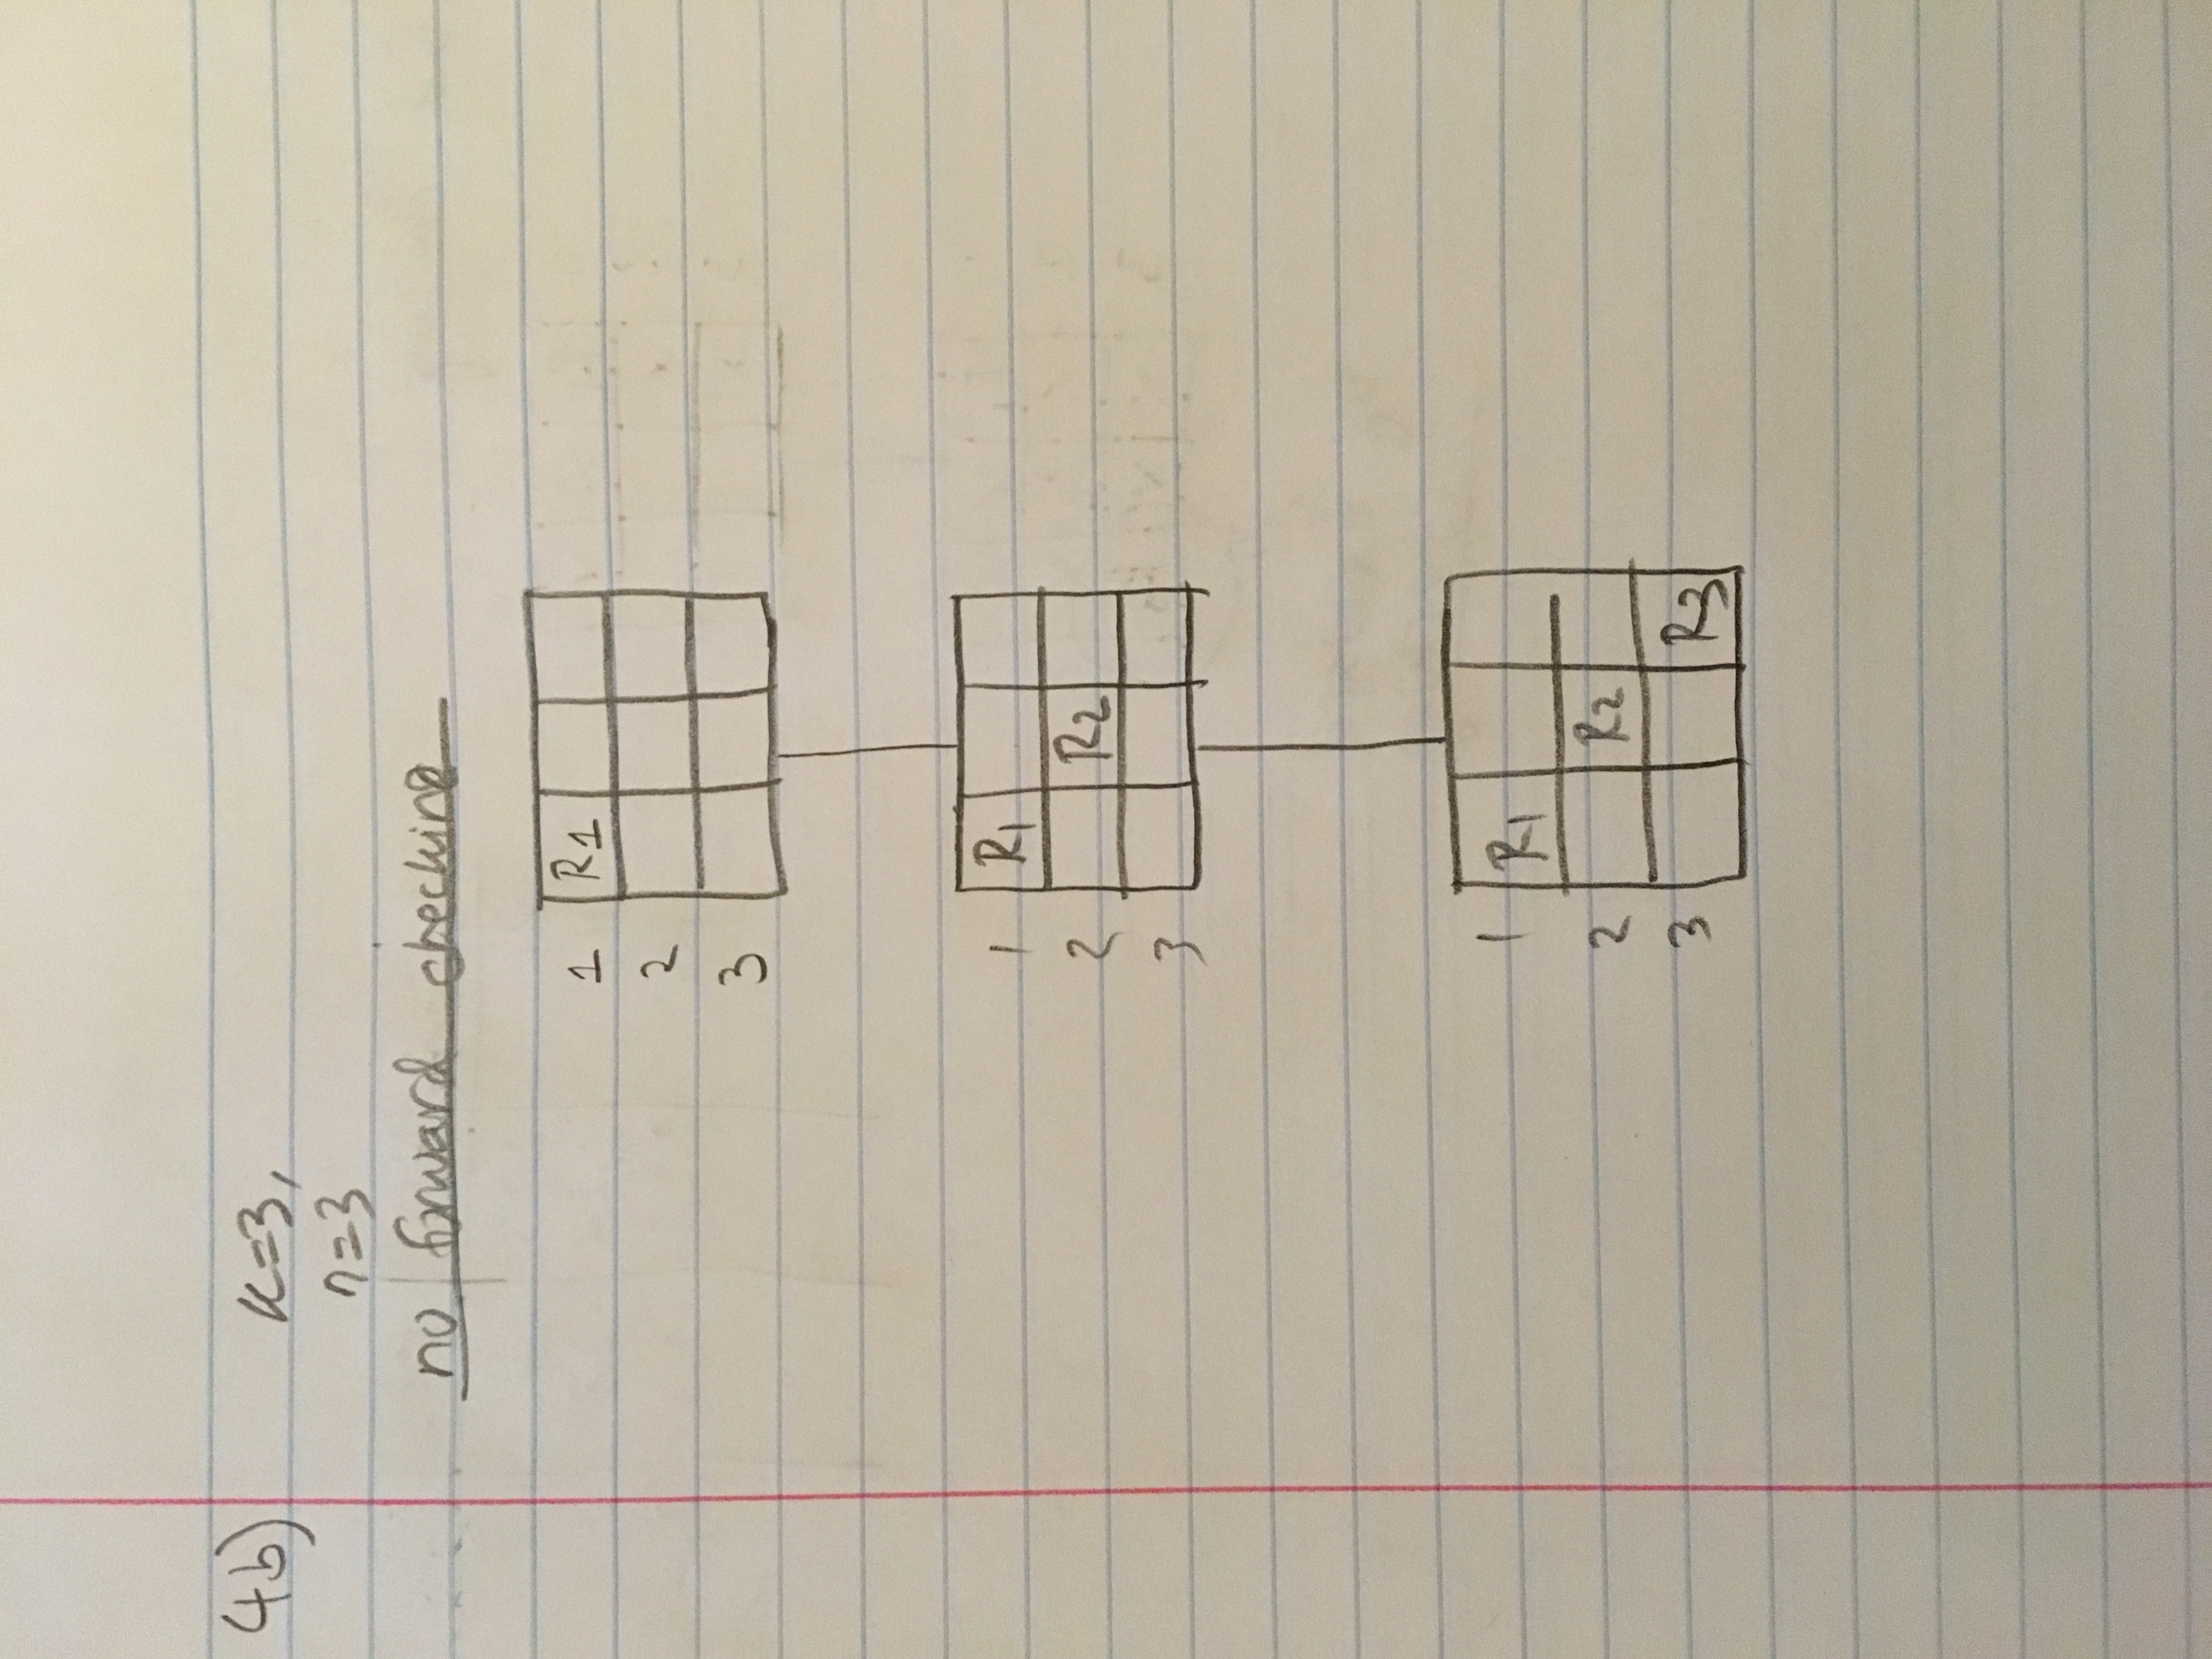
\includegraphics[width=\linewidth]{nofwd.JPG}
\end{figure}

\subsection{Part C: With forward checking}
\begin{figure}[H]
    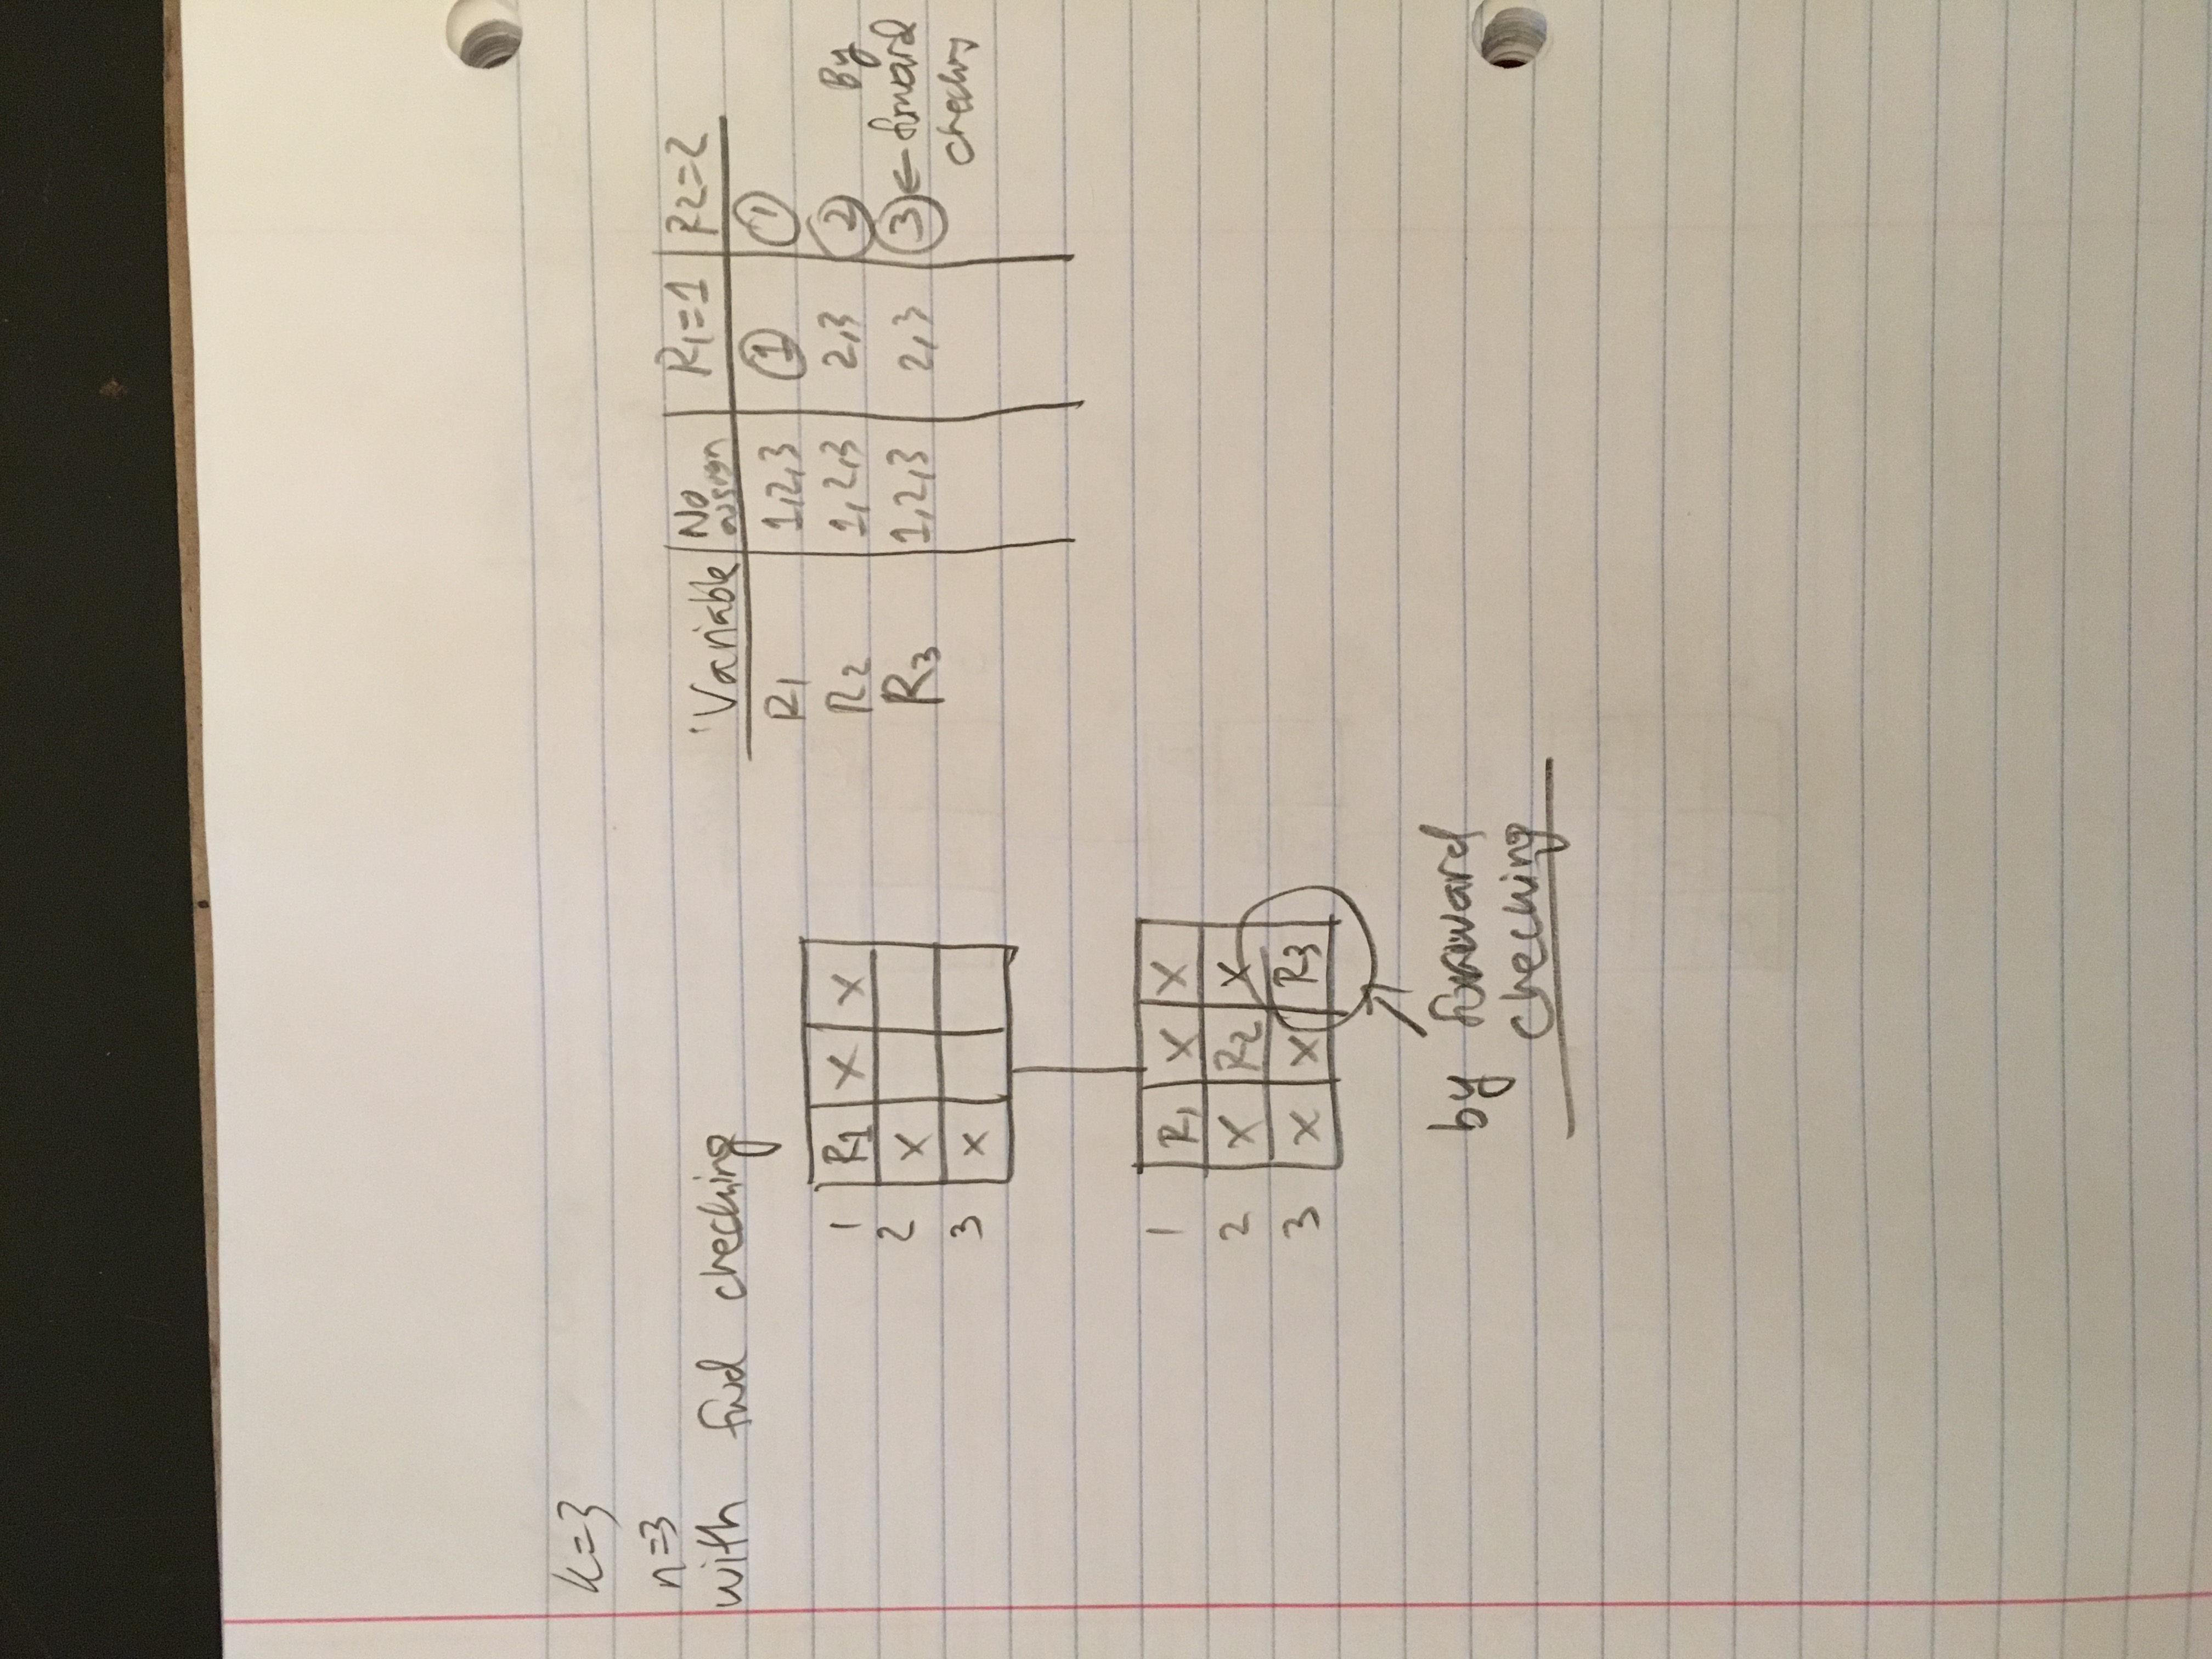
\includegraphics[width=\linewidth]{fwd.JPG}
\end{figure}

With forward checking we can immediately assign R3 without requiring an additional call.

\end{document}
